\chapter{Arhitektura i dizajn sustava}
		%komentar
		\textbf{\textit{dio 1. revizije}}\\

		\textit{ Potrebno je opisati stil arhitekture te identificirati: podsustave, preslikavanje na radnu platformu, spremišta podataka, mrežne protokole, globalni upravljački tok i sklopovsko-programske zahtjeve. Po točkama razraditi i popratiti odgovarajućim skicama:}
	\begin{itemize}
		\item 	\textit{izbor arhitekture temeljem principa oblikovanja pokazanih na predavanjima (objasniti zašto ste baš odabrali takvu arhitekturu)}
		\item 	\textit{organizaciju sustava s najviše razine apstrakcije (npr. klijent-poslužitelj, baza podataka, datotečni sustav, grafičko sučelje)}
		\item 	\textit{organizaciju aplikacije (npr. slojevi frontend i backend, MVC arhitektura) }		
	\end{itemize}

	
		

		

				
		\section{Baza podataka}
			
			\textbf{\textit{dio 1. revizije}}\\
			
		\textit{Potrebno je opisati koju vrstu i implementaciju baze podataka ste odabrali, glavne komponente od kojih se sastoji i slično.}
		
			\subsection{Opis tablica}
			

				\textit{Svaku tablicu je potrebno opisati po zadanom predlošku. Lijevo se nalazi točno ime varijable u bazi podataka, u sredini se nalazi tip podataka, a desno se nalazi opis varijable. Svjetlozelenom bojom označite primarni ključ. Svjetlo plavom označite strani ključ}
				
				
				\textbf{Users}\hspace{1cm}  Ova tablica sadrži sve relevantne informacije za korisnike aplikacije. Sadrži atribute: UserId, Username, email i verified(boolean atribut koji nam govori je li korisnik verificirao svoj račun). Tablica je u vezi \textit{One-to-One} s tablicom Companies i u vezi \textit{One-to-Many} je s tablicom Locations. 

                
                \begin{longtblr}[
					label=none,
					entry=none
					]{
						width = \textwidth,
						colspec={|X[6,l]|X[6, l]|X[20, l]|}, 
						rowhead = 1,
					} %definicija širine tablice, širine stupaca, poravnanje i broja redaka naslova tablice
					\hline {\textbf{Users}}	 \\ \hline[3pt]
					\SetCell{LightGreen}UserId & VARCHAR	&  	Hashirani string jedinstven za svakog korisnika  	\\ \hline
					Username	& VARCHAR & Nadimak pod kojim će se korisnik predstavljati u aplikaciji  	\\ \hline 
					email & VARCHAR &  E-mail adresa korisnika \\ \hline 
					Verified & BOOLEAN	&  True ako je korisnik potvrdio registraciju preko maila, inače False		\\ \hline  
				\end{longtblr}
                \textbf{Locations} \hspace{1cm} Ova tablica sadrži informacije o lokacijama dodanih od strane korisnika. Sadrži atribute: Ime lokacije, id korisnika koji je dodao lokaciju, status prikladnosti i koordinate. U vezi  \textit{Many-to-One} je s tablicom Users.
                \begin{longtblr}[
					label=none,
					entry=none
					]{
						width = \textwidth,
						colspec={|X[6,l]|X[6, l]|X[20, l]|}, 
						rowhead = 1,
					} %definicija širine tablice, širine stupaca, poravnanje i broja redaka naslova tablice
					\hline {\textbf{Locations}}	 \\ \hline[3pt]
					\SetCell{LightGreen}Name & VARCHAR	&  Ime lokacije  	\\ \hline
					\SetCell{LightBlue} UserId	& VARCHAR &  Hashirani string niz jedinstven za korisnika koji je dodao lokaciju 	\\ \hline  
					Prikladna & BOOLEAN	&  True ako je prikladna za ljubimce, inače False		\\ \hline 
                    Coordinates & VARCHAR &  Koordinate lokacije \\ \hline 
				\end{longtblr}
                \textbf{Companies} \hspace{1cm} Ova tablica sadrži informacije o dodanim obrtima. Posjeduje atribute: OIB obrta, Id vlasnika obrta, adresu, naziv obrta, kojoj kategoriji pripada i kratki opis obrta.  U vezi  \textit{One-to-One} je s tablicom Users.
                \begin{longtblr}[
					label=none,
					entry=none
					]{
						width = \textwidth,
						colspec={|X[6,l]|X[6, l]|X[20, l]|}, 
						rowhead = 1,
					} %definicija širine tablice, širine stupaca, poravnanje i broja redaka naslova tablice
					\hline {\textbf{Companies}}	 \\ \hline[3pt]
					\SetCell{LightGreen}OIB & VARCHAR	&  Niz od 11 znamenki karakterističan za tu pravnu osobu  	\\ \hline
					\SetCell{LightBlue} OwnerId	& VARCHAR &  Hashirani string niz jedinstven za korisnika koji je ujedino i vlasnik obrta 	\\ \hline  
					Adresa & VARCHAR	&  Adresa obrta	\\ \hline 
                    Ime & VARCHAR &  Ime obrta \\ \hline 
                    Tip & VARCHAR &  Kategorija kojoj obrt pripada \\ \hline 
                    Opis & VARCHAR &  Kratki opis obrta \\ \hline 
				\end{longtblr}

                
				
				
			
			\subsection{Dijagram baze podataka}
				\textit{ U ovom potpoglavlju potrebno je umetnuti dijagram baze podataka. Primarni i strani ključevi moraju biti označeni, a tablice povezane. Bazu podataka je potrebno normalizirati. Podsjetite se kolegija "Baze podataka".}
                %oznaci kljuceve
                \begin{figure}[H]
			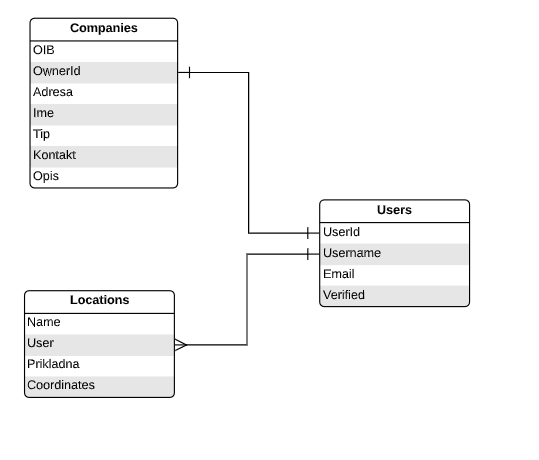
\includegraphics[scale=1.2]{slike/Baza.png}
			\centering
			\caption{Dijagram baze podataka}
			\label{fig:promjene}
		          \end{figure}
			
			\eject
			
		\section{Dijagram razreda}
		
			\textit{Potrebno je priložiti dijagram razreda s pripadajućim opisom. Zbog preglednosti je moguće dijagram razlomiti na više njih, ali moraju biti grupirani prema sličnim razinama apstrakcije i srodnim funkcionalnostima.}\\
			
			\textbf{\textit{dio 1. revizije}}\\
			
			\textit{Prilikom prve predaje projekta, potrebno je priložiti potpuno razrađen dijagram razreda vezan uz \textbf{generičku funkcionalnost} sustava. Ostale funkcionalnosti trebaju biti idejno razrađene u dijagramu sa sljedećim komponentama: nazivi razreda, nazivi metoda i vrste pristupa metodama (npr. javni, zaštićeni), nazivi atributa razreda, veze i odnosi između razreda.}\\
			
			\textbf{\textit{dio 2. revizije}}\\			
			
			\textit{Prilikom druge predaje projekta dijagram razreda i opisi moraju odgovarati stvarnom stanju implementacije}
			
			
			
			\eject
		
		\section{Dijagram stanja}
			
			
			\textbf{\textit{dio 2. revizije}}\\
			
			\textit{Potrebno je priložiti dijagram stanja i opisati ga. Dovoljan je jedan dijagram stanja koji prikazuje \textbf{značajan dio funkcionalnosti} sustava. Na primjer, stanja korisničkog sučelja i tijek korištenja neke ključne funkcionalnosti jesu značajan dio sustava, a registracija i prijava nisu. }
			
			
			\eject 
		
		\section{Dijagram aktivnosti}
			
			\textbf{\textit{dio 2. revizije}}\\
			
			 \textit{Potrebno je priložiti dijagram aktivnosti s pripadajućim opisom. Dijagram aktivnosti treba prikazivati značajan dio sustava.}
			
			\eject
		\section{Dijagram komponenti}
		
			\textbf{\textit{dio 2. revizije}}\\
		
			 \textit{Potrebno je priložiti dijagram komponenti s pripadajućim opisom. Dijagram komponenti treba prikazivati strukturu cijele aplikacije.}